\documentclass[a0,portrait]{a0poster}

\usepackage{multicol}
\columnsep=100pt
\columnseprule=3pt

\usepackage[svgnames]{xcolor}

\usepackage{times}
\usepackage{palatino}
\usepackage[none]{hyphenat}
\usepackage{graphicx}
\graphicspath{{figures/}}
\usepackage{booktabs}
\usepackage[font=small,labelfont=bf]{caption}
\usepackage{amsfonts, amsmath, amsthm, amssymb}
\usepackage{wrapfig}
\usepackage{lipsum,adjustbox}
\usepackage[absolute,overlay]{textpos}
\usepackage{multirow}
\usepackage{titlesec}
\usepackage[inline]{enumitem}
\usepackage{url}
\usepackage{tikz,pgfplots,pgfplotstable}
\usepackage{tikz-dependency}
\usepackage[most]{tcolorbox}
\usepackage[charter]{mathdesign}
\def\rmdefault{bch} % not scaled
\def\ttdefault{blg}
\def\scdefault{sc}
\usetikzlibrary{arrows.meta}
\captionsetup{labelformat=empty}

\begin{document}

\begin{center}
	\veryHuge \color{NavyBlue} \textbf{Universal Dependency Parsing \\
	with a General Transition-Based DAG Parser}
\end{center}
\begin{minipage}[b]{0.57\linewidth}
\LARGE \textbf{Daniel Hershcovich}\textsuperscript{1,2} \&
	   \textbf{Omri Abend}\textsuperscript{2} \&
	   \textbf{Ari Rappoport}\textsuperscript{2} \\[0.5cm]
\large $^1$The Edmond and Lily Safra Center for Brain Sciences \\
  $^2$School of Computer Science and Engineering
  \setlength{\columnseprule}{0pt}
  \setlength\multicolsep{-20pt}
  \begin{multicols}{2}
  The Hebrew University of Jerusalem \\
  \texttt{\{danielh,oabend,arir\}@cs.huji.ac.il}
  \end{multicols}
\end{minipage}
\hfill
\begin{minipage}[b]{.1\linewidth}

\includegraphics[width=\linewidth]{elsc_logo.png}
\end{minipage}
\begin{minipage}[b]{.18\linewidth}

\includegraphics[width=\linewidth]{huji_banner.png}

\includegraphics[width=1.04\linewidth]{cse_banner.jpg}
\end{minipage}
\begin{minipage}[b]{.07\linewidth}

\includegraphics[width=\linewidth]{huji_logo.jpg}
\end{minipage}

\vspace{1cm}
\titlespacing*{\section}{0pt}{8mm}{5mm}

%----------------------------------------------------------------------------------------


\begin{adjustbox}{margin=5mm,frame,minipage=.71\linewidth,center}
\Large\color{Navy}
Learning to parse \textbf{enhanced dependencies} jointly with basic Universal Dependency Parsing.
\end{adjustbox}

\begin{center}
\url{github.com/CoNLL-UD-2018/HUJI}
\end{center}

\begin{multicols}{2}


\color{Black}
\tcbset{
    colback=gray!40,
    width=1.05\columnwidth,
    colframe=white
    }
    
\begin{tcolorbox}
We extend \textbf{TUPA} \cite{hershcovich2017a,hershcovich2018multitask}, a general DAG parser
originally designed for UCCA:
transition-based parser supporting reentrancy (DAG),
discontinuity (non-projectivity) and non-terminal nodes.

\vfill

\begin{adjustbox}{margin=3mm,frame}
\textsc{Shift, Reduce, Node$_X$, Right-Edge$_X$, Left-Enhanced$_X$, Right-Enhanced$_X$, Swap, Finish}
\end{adjustbox}

\vfill

\begin{center}
\large
   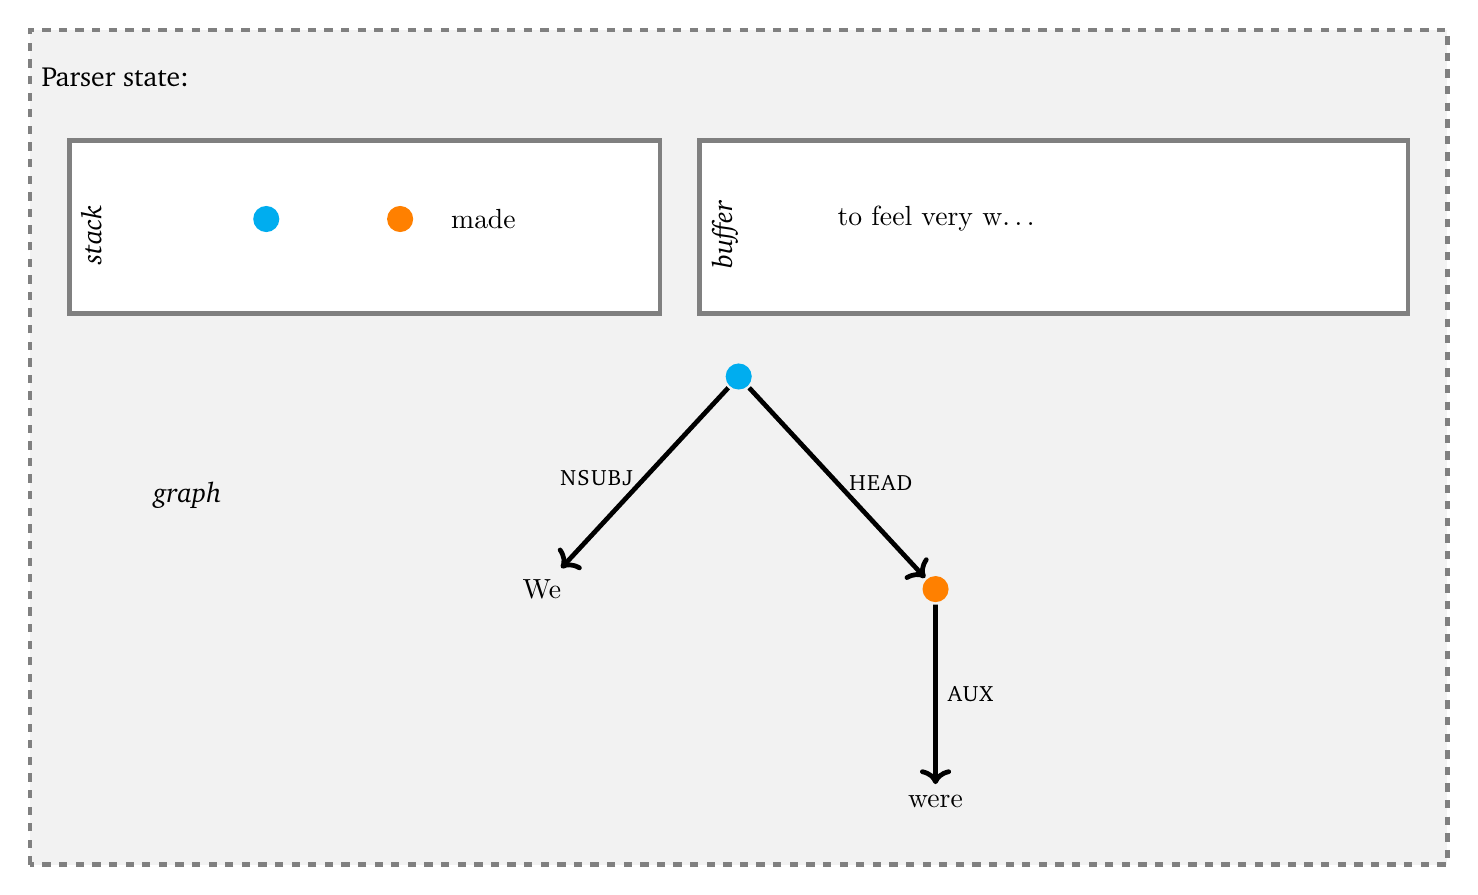
\begin{tikzpicture}[level distance=27mm, sibling distance=5cm,line width=.6mm,-{Latex[length=3mm]}]
   \draw[color=gray,dashed,fill=lightgray!20] (0,-5) rectangle (18,5.6);
   \node[anchor=west] at (0,5) {\normalsize Parser state:};
   \draw[color=gray,fill=white] (.5,2) rectangle (8,4.2);
   \node[anchor=north,rotate=90] at (.5,3) {\normalsize \textit{stack}};
   \node[fill=cyan, circle] at (3,3.2) {};
   \node[fill=orange, circle] at (4.7,3.2) {};
   \node[anchor=west] at (5.2,3.2) {\ttfamily made};
   \draw[color=gray,fill=white] (8.5,2) rectangle (17.5,4.2);
   \node[anchor=north,rotate=90] at (8.51,3) {\normalsize \textit{buffer}};
   \node[anchor=west] at (10.11,3.2) {\ttfamily to feel very w\ldots};
   \node[anchor=north] at (2,0) {\textit{graph}};
   \node[fill=cyan, circle] at (9,1.2) {}   
     child {node  {\ttfamily We} edge from parent [->] node[left] {\textsc{nsubj}}}
     child {node [fill=orange, circle] {}
     {
       child {node {\ttfamily were} edge from parent [->] node[right] {\textsc{aux}}}
     } edge from parent [->] node[right] {\textsc{head}} };
   \end{tikzpicture}
   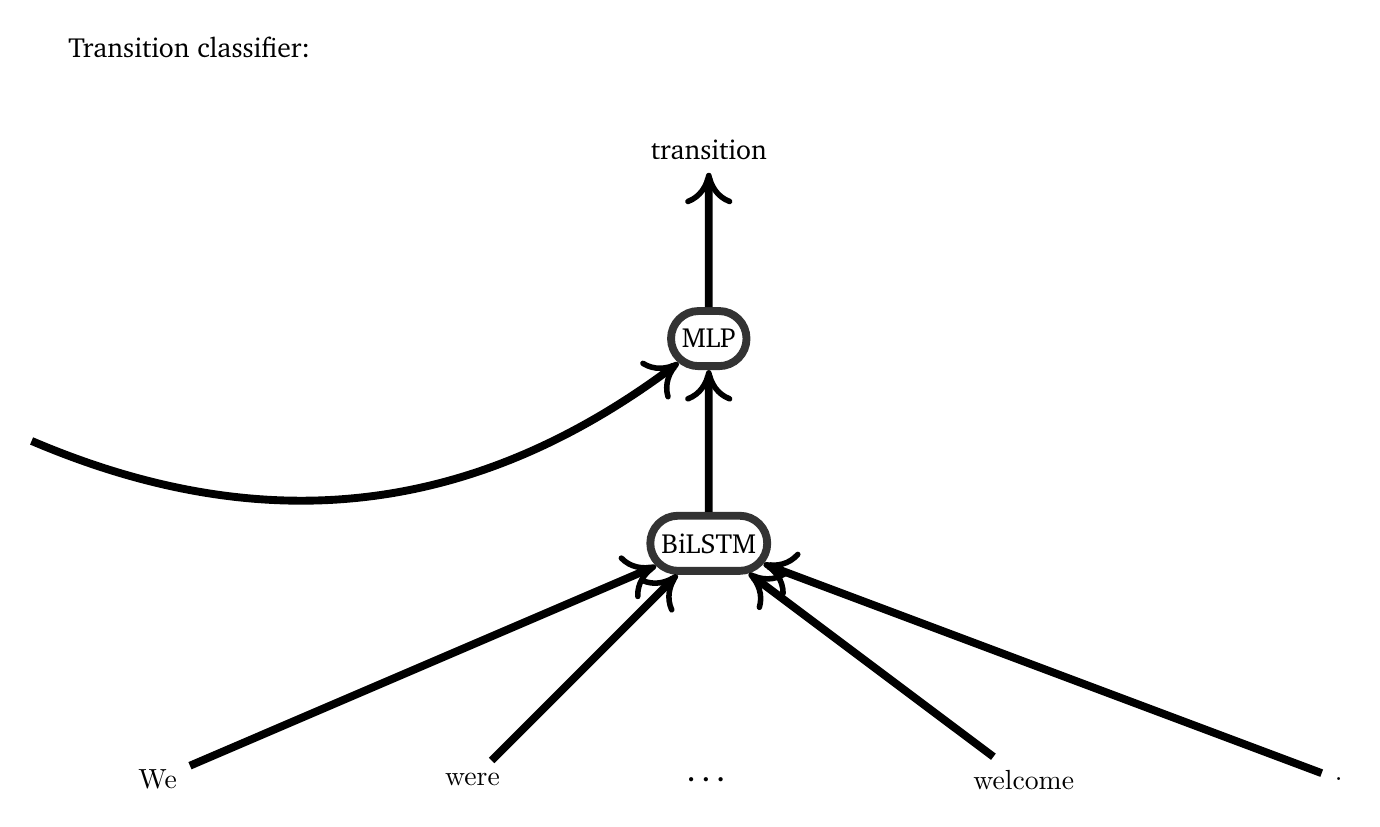
\begin{tikzpicture}[->,line width=1mm]
   \node[anchor=west] at (-1.3,11.3) {\normalsize Transition classifier:};
   \tikzstyle{main}=[rounded rectangle, minimum size=7mm, draw=black!80, node distance=12mm,fill=white]
   \node[main] (specific) at (7,5) {BiLSTM};
   \foreach \i/\word in {0/{We},4/{were},11/{welcome},15/{.}} {
       \node (x\i) at (\i,2) {\ttfamily\word};
       \path[arrows={->[line width=2pt,length=4mm,width=6mm]}] (x\i) edge (specific);
   }
    \node (x4) at (7,2) {\large\ldots};
    \node[main] (mlp) at (7,7.6) {MLP};
    \path[arrows={->[line width=2pt,length=4mm,width=6mm]}] (specific) edge (mlp);
    \coordinate (state) at (-1.6,6.3);
    \path[arrows={->[line width=2pt,length=4mm,width=6mm]}] (state) edge [bend right] (mlp);
    \node (transition) at (7,10) {transition};
    \path[arrows={->[line width=2pt,length=4mm,width=6mm]}] (mlp) edge node[right] {} (transition);
   \end{tikzpicture}
\end{center}

\vfill

Example:

\scalebox{.9}{
\begin{minipage}{.538\columnwidth}
	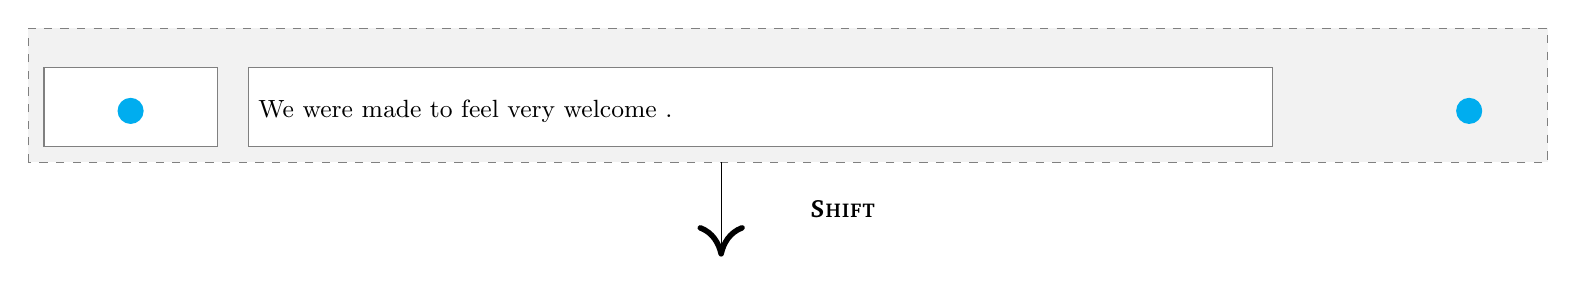
\begin{tikzpicture}[level distance=15mm, sibling distance=4cm, font=\small]
	\draw[color=gray,dashed,fill=lightgray!20] (.2,-.2) rectangle (19.5,1.5);
	\draw[color=gray,fill=white] (.4,0) rectangle (2.6,1);
	\node[fill=cyan, circle] at (1.5,.45) {};
	\draw[color=gray,fill=white] (3,0) rectangle (16,1);
	\node[anchor=west] at (3,.45) {\ttfamily We were made to feel very welcome .};
	\node[fill=cyan, circle] at (18.5,.45) {};
	\node[anchor=west] at (10,-.8) {\bf\small\textsc{Shift}};
	\draw[arrows={->[line width=2pt,length=4mm,width=6mm]}] (9,-.2) -- (9,-1.4);
	\end{tikzpicture}
	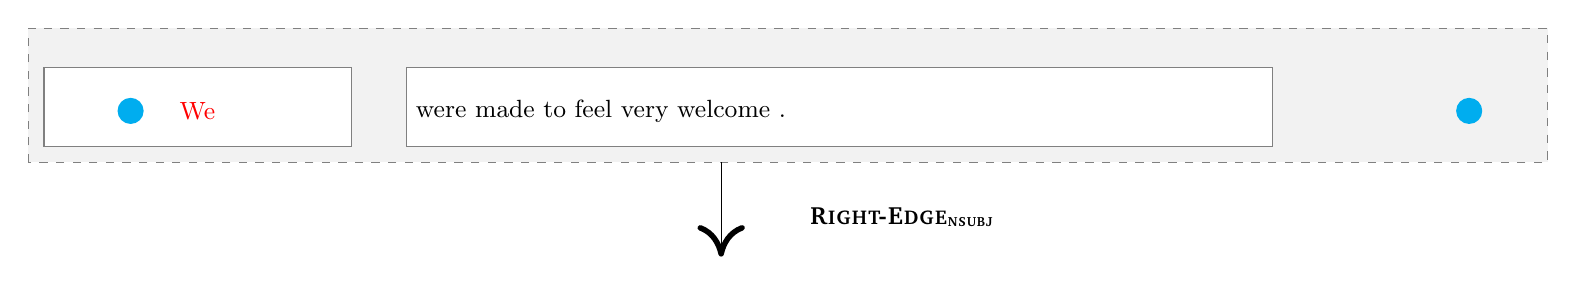
\begin{tikzpicture}[level distance=15mm, sibling distance=4cm, font=\small]
	\draw[color=gray,dashed,fill=lightgray!20] (.2,-.2) rectangle (19.5,1.5);
	\draw[color=gray,fill=white] (.4,0) rectangle (4.3,1);
	\node[fill=cyan, circle] at (1.5,.45) {};
	\node[color=red,anchor=west] at (2,.45) {\ttfamily We};
	\draw[color=gray,fill=white] (5,0) rectangle (16,1);
	\node[anchor=west] at (5,.45) {\ttfamily were made to feel very welcome .};
	\node[fill=cyan, circle] at (18.5,.45) {};
	\node[anchor=west] at (10,-.9) {\bf\small\textsc{Right-Edge\textsubscript {nsubj}}};
	\draw[arrows={->[line width=2pt,length=4mm,width=6mm]}] (9,-.2) -- (9,-1.4);
	\end{tikzpicture}
	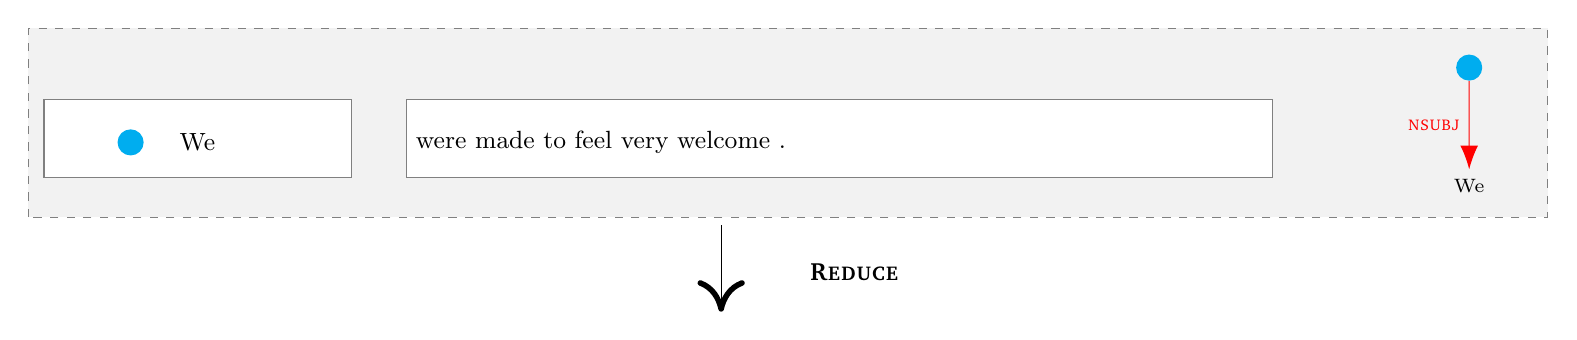
\begin{tikzpicture}[level distance=15mm, sibling distance=4cm, font=\small, -{Latex[length=3mm]}]
	\draw[color=gray,dashed,fill=lightgray!20] (.2,-.5) rectangle (19.5,1.9);
	\draw[color=gray,fill=white] (.4,0) rectangle (4.3,1);
	\node[fill=cyan, circle] at (1.5,.45) {};
	\node[anchor=west] at (2,.45) {\ttfamily We};
	\draw[color=gray,fill=white] (5,0) rectangle (16,1);
	\node[anchor=west] at (5,.45) {\ttfamily were made to feel very welcome .};
	\node[fill=cyan, circle] at (18.5,1.4) {}
	  child {node[font=\scriptsize] {\ttfamily We} edge from parent [red] node[font=\scriptsize,left] {\textsc{nsubj}}};
	\node[anchor=west] at (10,-1.2) {\bf\small\textsc{Reduce}};
	\draw[arrows={->[line width=2pt,length=4mm,width=6mm]}] (9,-.6) -- (9,-1.7);
	\end{tikzpicture}
	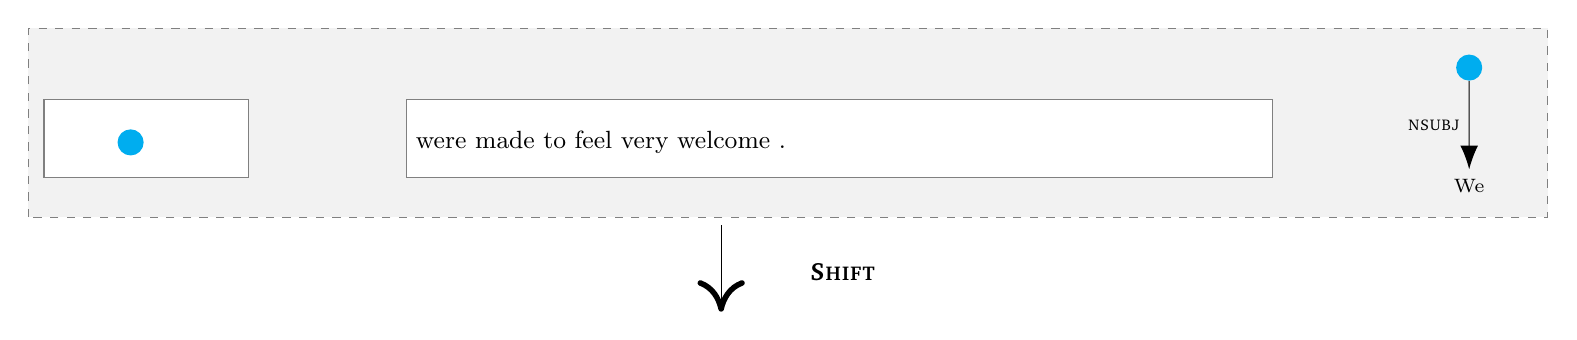
\begin{tikzpicture}[level distance=15mm, sibling distance=4cm, font=\small, -{Latex[length=3mm]}]
	\draw[color=gray,dashed,fill=lightgray!20] (.2,-.5) rectangle (19.5,1.9);
	\draw[color=gray,fill=white] (.4,0) rectangle (3,1);
	\node[fill=cyan, circle] at (1.5,.45) {};
	\draw[color=gray,fill=white] (5,0) rectangle (16,1);
	\node[anchor=west] at (5,.45) {\ttfamily were made to feel very welcome .};
	\node[fill=cyan, circle] at (18.5,1.4) {}
	  child {node[font=\scriptsize] {\ttfamily We} edge from parent node[font=\scriptsize,left] {\textsc{nsubj}}};
	\node[anchor=west] at (10,-1.2) {\bf\small\textsc{Shift}};
	\draw[arrows={->[line width=2pt,length=4mm,width=6mm]}] (9,-.6) -- (9,-1.7);
	\end{tikzpicture}
	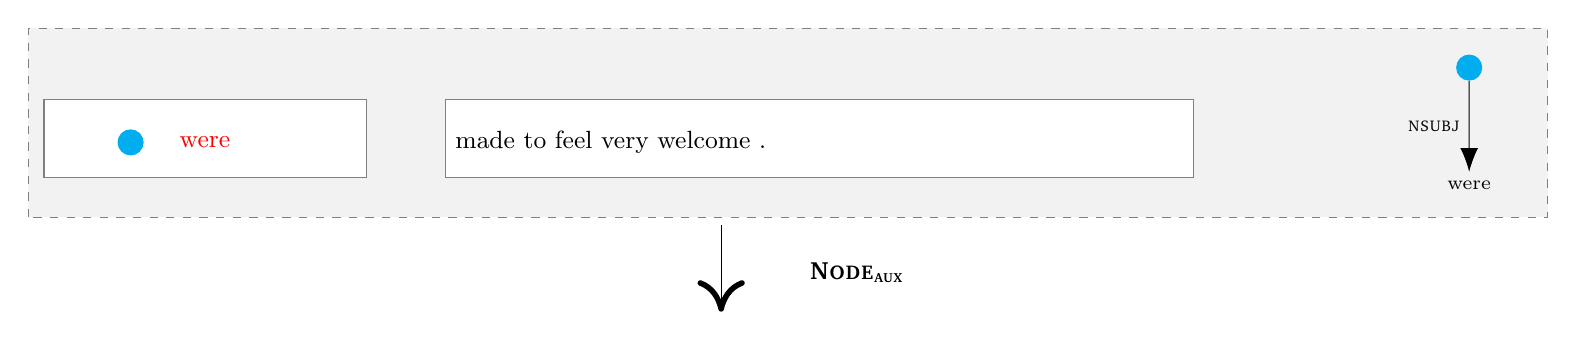
\begin{tikzpicture}[level distance=15mm, sibling distance=4cm, font=\small, -{Latex[length=3mm]}]
	\draw[color=gray,dashed,fill=lightgray!20] (.2,-.5) rectangle (19.5,1.9);
	\draw[color=gray,fill=white] (.4,0) rectangle (4.5,1);
	\node[fill=cyan, circle] at (1.5,.45) {};
	\node[color=red,anchor=west] at (2,.45) {\ttfamily were};
	\draw[color=gray,fill=white] (5.5,0) rectangle (15,1);
	\node[anchor=west] at (5.5,.45) {\ttfamily made to feel very welcome .};
	\node[fill=cyan, circle] at (18.5,1.4) {}
	  child {node[font=\scriptsize] {\ttfamily were} edge from parent node[font=\scriptsize,left] {\textsc{nsubj}}};
	\node[anchor=west] at (10,-1.2) {\bf\small\textsc{Node\textsubscript {aux}}};
	\draw[arrows={->[line width=2pt,length=4mm,width=6mm]}] (9,-.6) -- (9,-1.7);
	\end{tikzpicture}
	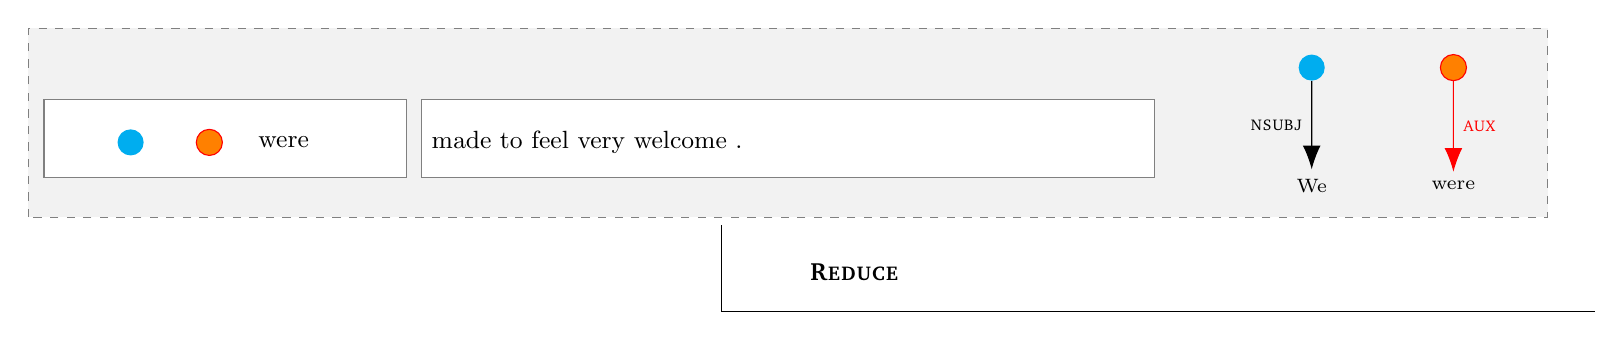
\begin{tikzpicture}[level distance=15mm, sibling distance=4cm, font=\small, -{Latex[length=3mm]}]
	\draw[color=gray,dashed,fill=lightgray!20] (.2,-.5) rectangle (19.5,1.9);
	\draw[color=gray,fill=white] (.4,0) rectangle (5,1);
	\node[fill=cyan, circle] at (1.5,.45) {};
	\node[fill=orange, draw=red, circle] at (2.5,.45) {};
	\node[anchor=west] at (3,.45) {\ttfamily were};
	\draw[color=gray,fill=white] (5.2,0) rectangle (14.5,1);
	\node[anchor=west] at (5.2,.45) {\ttfamily made to feel very welcome .};
	\node[fill=cyan, circle] at (16.5,1.4) {}
	  child {node[font=\scriptsize] {\ttfamily We} edge from parent node[font=\scriptsize,left] {\textsc{nsubj}}};
	\node[fill=orange, draw=red, circle] at (18.3,1.4) {}
	  child {node[font=\scriptsize] {\ttfamily were} edge from parent [red] node[font=\scriptsize,right] {\textsc{aux}}};
	\node[anchor=west] at (10,-1.2) {\bf\small\textsc{Reduce}};
	\draw[arrows={-[line width=2pt,length=4mm,width=6mm]}] (9,-.6) -- (9,-1.7);
	\draw[arrows={-[line width=2pt,length=4mm,width=6mm]}] (9,-1.7) -- (20.1,-1.7);
	\end{tikzpicture}
\end{minipage}
\hspace{1pt}
\begin{minipage}{8mm}
    \vspace{5mm}
    \begin{tikzpicture}
    	\draw[arrows={-[line width=2pt,length=4mm,width=6mm]}] (0,0) -- (0,20);
    	\draw[arrows={->[line width=2pt,length=4mm,width=6mm]}] (0,20) -- (1,20);
	\end{tikzpicture}
\end{minipage}
\begin{minipage}{.4\columnwidth}
	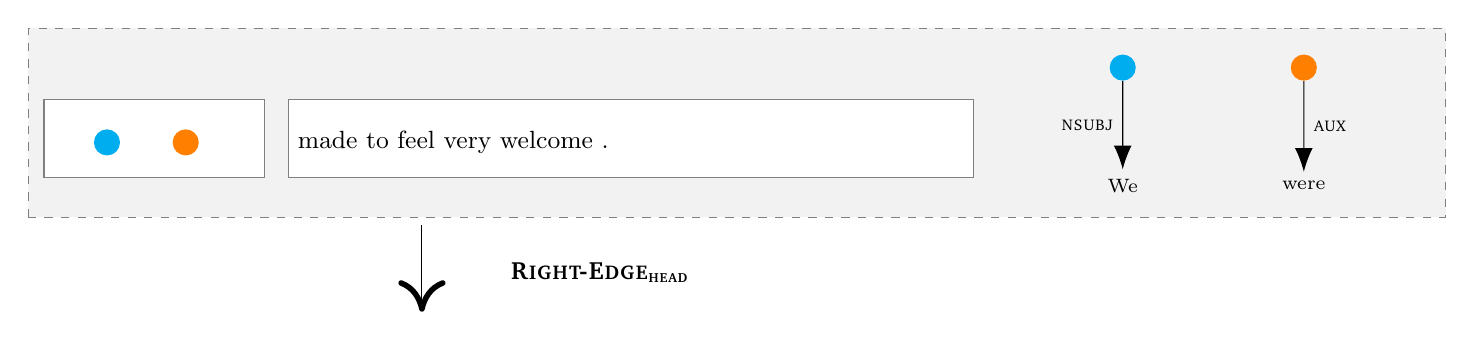
\begin{tikzpicture}[level distance=15mm, sibling distance=4cm, font=\small, -{Latex[length=3mm]}]
	\draw[color=gray,dashed,fill=lightgray!20] (0,-.5) rectangle (18,1.9);
	\draw[color=gray,fill=white] (0.2,0) rectangle (3,1);
	\node[fill=cyan, circle] at (1,.45) {};
	\node[fill=orange, circle] at (2,.45) {};
	\draw[color=gray,fill=white] (3.3,0) rectangle (12,1);
	\node[anchor=west] at (3.3,.45) {\ttfamily made to feel very welcome .};
	\node[fill=cyan, circle] at (13.9,1.4) {}
	  child {node[font=\scriptsize] {\ttfamily We} edge from parent node[font=\scriptsize,left] {\textsc{nsubj}}};
	\node[fill=orange, circle] at (16.2,1.4) {}
	  child {node[font=\scriptsize] {\ttfamily were} edge from parent node[font=\scriptsize,right] {\textsc{aux}}};
	\node[anchor=west] at (6,-1.2) {\bf\small\textsc{Right-Edge\textsubscript {head}}};
	\draw[arrows={->[line width=2pt,length=4mm,width=6mm]}] (5,-.6) -- (5,-1.7);
	\end{tikzpicture}
	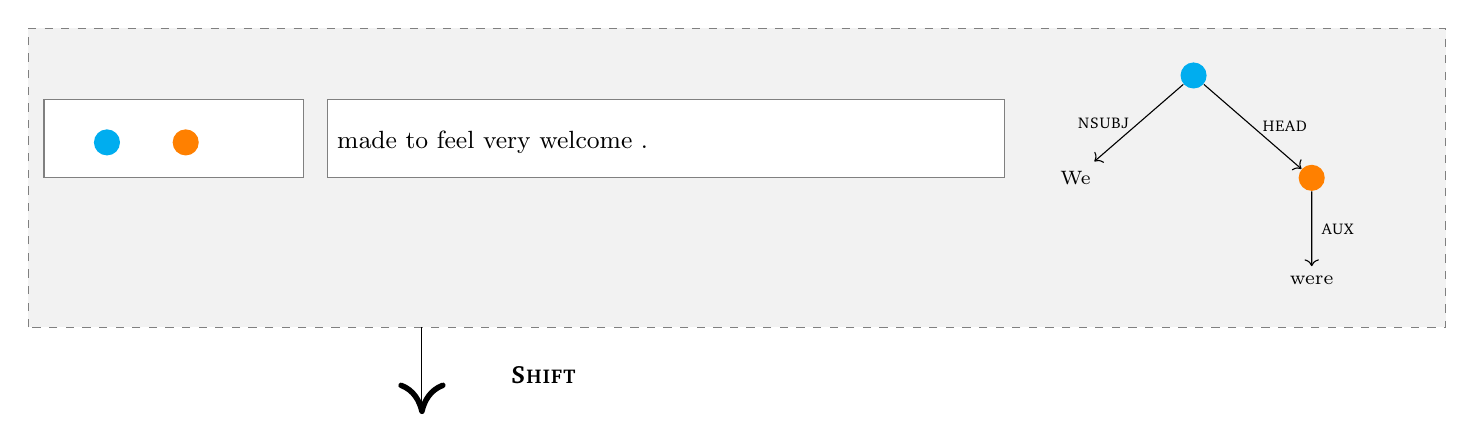
\begin{tikzpicture}[level distance=13mm, sibling distance=3cm, font=\small, -{Latex[length=3mm]}]
	\draw[color=gray,dashed,fill=lightgray!20] (0,-1.9) rectangle (18,1.9);
	\draw[color=gray,fill=white] (0.2,0) rectangle (3.5,1);
	\node[fill=cyan, circle] at (1,.45) {};
	\node[fill=orange, circle] at (2,.45) {};
	\draw[color=gray,fill=white] (3.8,0) rectangle (12.4,1);
	\node[anchor=west] at (3.8,.45) {\ttfamily made to feel very welcome .};
   \node[fill=cyan, circle] at (14.8,1.3) {}   
     child {node[font=\scriptsize] {\ttfamily We} edge from parent [->] node[font=\scriptsize,left] {\textsc{nsubj}}}
     child {node [fill=orange, circle] {}
     {
       child {node[font=\scriptsize] {\ttfamily were} edge from parent [->] node[font=\scriptsize,right] {\textsc{aux}}}
     } edge from parent [->] node[font=\scriptsize,right] {\textsc{head}} };
	\node[anchor=west] at (6,-2.5) {\bf\small\textsc{Shift}};
	\draw[arrows={->[line width=2pt,length=4mm,width=6mm]}] (5,-1.9) -- (5,-3);
	\end{tikzpicture}
	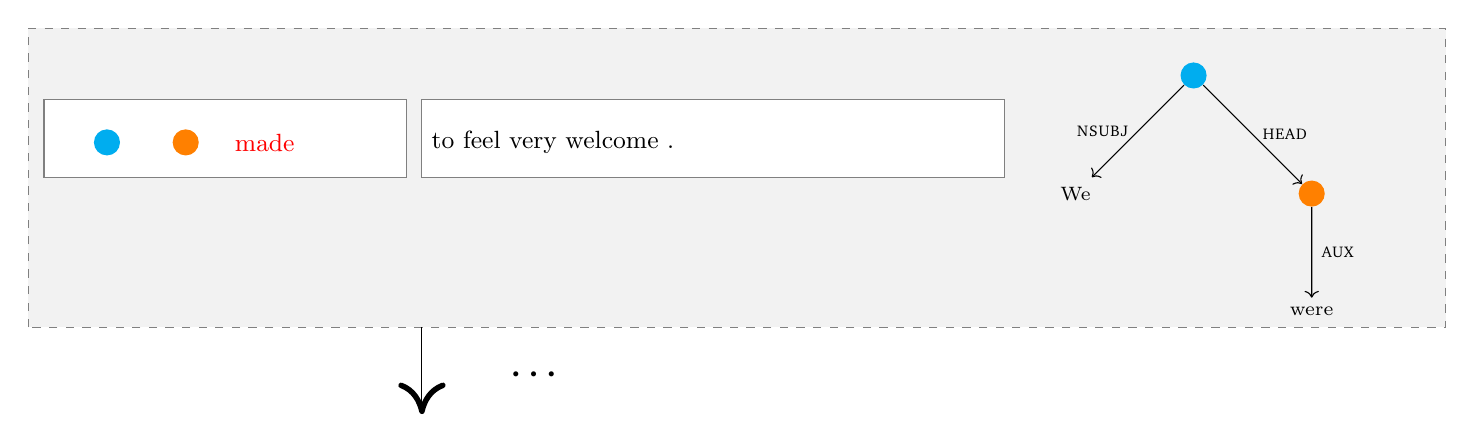
\begin{tikzpicture}[level distance=15mm, sibling distance=3cm, font=\small, -{Latex[length=3mm]}]
	\draw[color=gray,dashed,fill=lightgray!20] (0,-1.9) rectangle (18,1.9);
	\draw[color=gray,fill=white] (0.2,0) rectangle (4.8,1);
	\node[fill=cyan, circle] at (1,.45) {};
	\node[fill=orange, circle] at (2,.45) {};
	\node[color=red, anchor=west] at (2.5,.45) {\ttfamily made};
	\draw[color=gray,fill=white] (5,0) rectangle (12.4,1);
	\node[anchor=west] at (5,.45) {\ttfamily to feel very welcome .};
   \node[fill=cyan, circle] at (14.8,1.3) {}   
     child {node[font=\scriptsize] {\ttfamily We} edge from parent [->] node[font=\scriptsize,left] {\textsc{nsubj}}}
     child {node [fill=orange, circle] {}
     {
       child {node[font=\scriptsize] {\ttfamily were} edge from parent [->] node[font=\scriptsize,right] {\textsc{aux}}}
     } edge from parent [->] node[font=\scriptsize,right] {\textsc{head}} };
	\node[anchor=west] at (6,-2.5) {\Large \ldots};
	\draw[arrows={->[line width=2pt,length=4mm,width=6mm]}] (5,-1.9) -- (5,-3);
	\end{tikzpicture}
    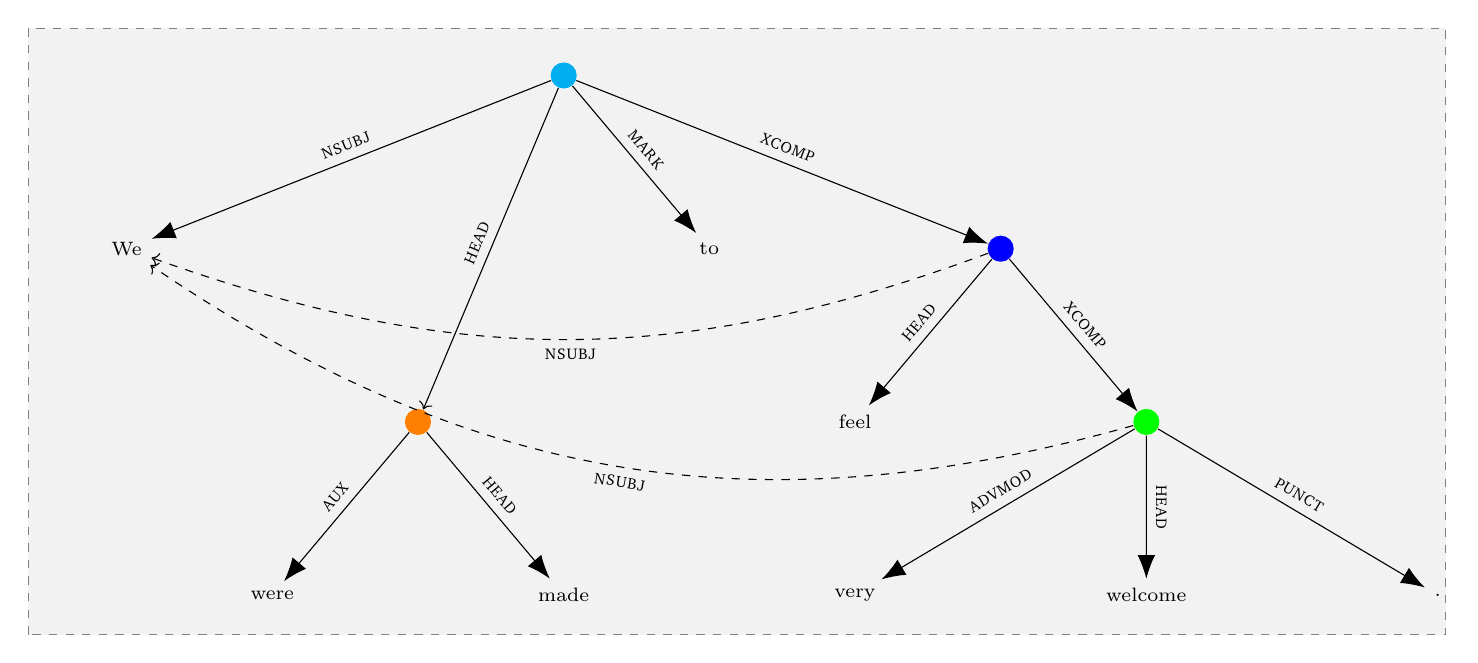
\begin{tikzpicture}[level distance=22mm, sibling distance=37mm, font=\small, -{Latex[length=3mm]}]
	\draw[color=gray,dashed,fill=lightgray!20] (0,-5.8) rectangle (18,1.9);
      \tikzstyle{word} = [color=black]
      \node (ROOT) at (6.8,1.3) [fill=cyan, circle] {}
        child {node (We) [font=\scriptsize\ttfamily] {We} edge from parent node[font=\scriptsize,midway,above,sloped] {\scriptsize \textsc{nsubj}}}
        child {node {}
        {
	        child {node (weremade) [fill=orange, circle] {}
	        {
	          child {node [font=\scriptsize\ttfamily] {were} edge from parent node[font=\scriptsize,midway,above,sloped] {\scriptsize \textsc{aux}}}
	          child {node [font=\scriptsize\ttfamily] {made} edge from parent node[font=\scriptsize,midway,above,sloped] {\scriptsize \textsc{head}}}
	        } edge from parent [draw=none]}
        } edge from parent [draw=none]}
        child {node [font=\scriptsize\ttfamily] {to} edge from parent node[font=\scriptsize,midway,above,sloped] {\scriptsize \textsc{mark}}}
        child {node (feelverywelcome) [fill=blue, circle] {}
        {
          child {node [font=\scriptsize\ttfamily] {feel} edge from parent node[font=\scriptsize,midway,above,sloped] {\scriptsize \textsc{head}}}
          child {node (verywelcome) [fill=green, circle] {}
          {
            child {node [font=\scriptsize\ttfamily] {very} edge from parent node[font=\scriptsize,midway,above,sloped] {\scriptsize \textsc{advmod}}}
            child {node [font=\scriptsize\ttfamily] {welcome} edge from parent node[font=\scriptsize,midway,above,sloped] {\scriptsize \textsc{head}}}
            child {node [font=\scriptsize\ttfamily] {.} edge from parent node[font=\scriptsize,midway,above,sloped] {\scriptsize \textsc{punct}}}
          } edge from parent node[font=\scriptsize,midway,above,sloped] {\scriptsize \textsc{xcomp}} }
        } edge from parent node[font=\scriptsize,midway,above,sloped] {\scriptsize \textsc{xcomp}} }
      ;
      \draw[->] (ROOT) to node [font=\scriptsize,midway,above,sloped] {\scriptsize \textsc{head}} (weremade);
      \draw[dashed,->,bend left=25] (verywelcome) to node [font=\scriptsize,midway,below,sloped] {\scriptsize \textsc{nsubj}} (We);
      \draw[dashed,->,bend left=20] (feelverywelcome) to node [font=\scriptsize,midway,below,sloped] {\scriptsize \textsc{nsubj}} (We);
    \end{tikzpicture}
\end{minipage}
}
\end{tcolorbox}

\vfill

\vspace{5mm}
{\color{Indigo}
\textbf{UCCA} \cite{abend2013universal}: Intuitive, cross-lingual, and modular semantic representation.
    \textit{Primary edges} form a tree. \textit{Remote edges} (dashed) allow reentrancy.
    Nodes represent scenes and concepts.}

\begin{minipage}{.55\columnwidth}
  \color{Indigo}
  \begin{center}
  \scalebox{.9}{
    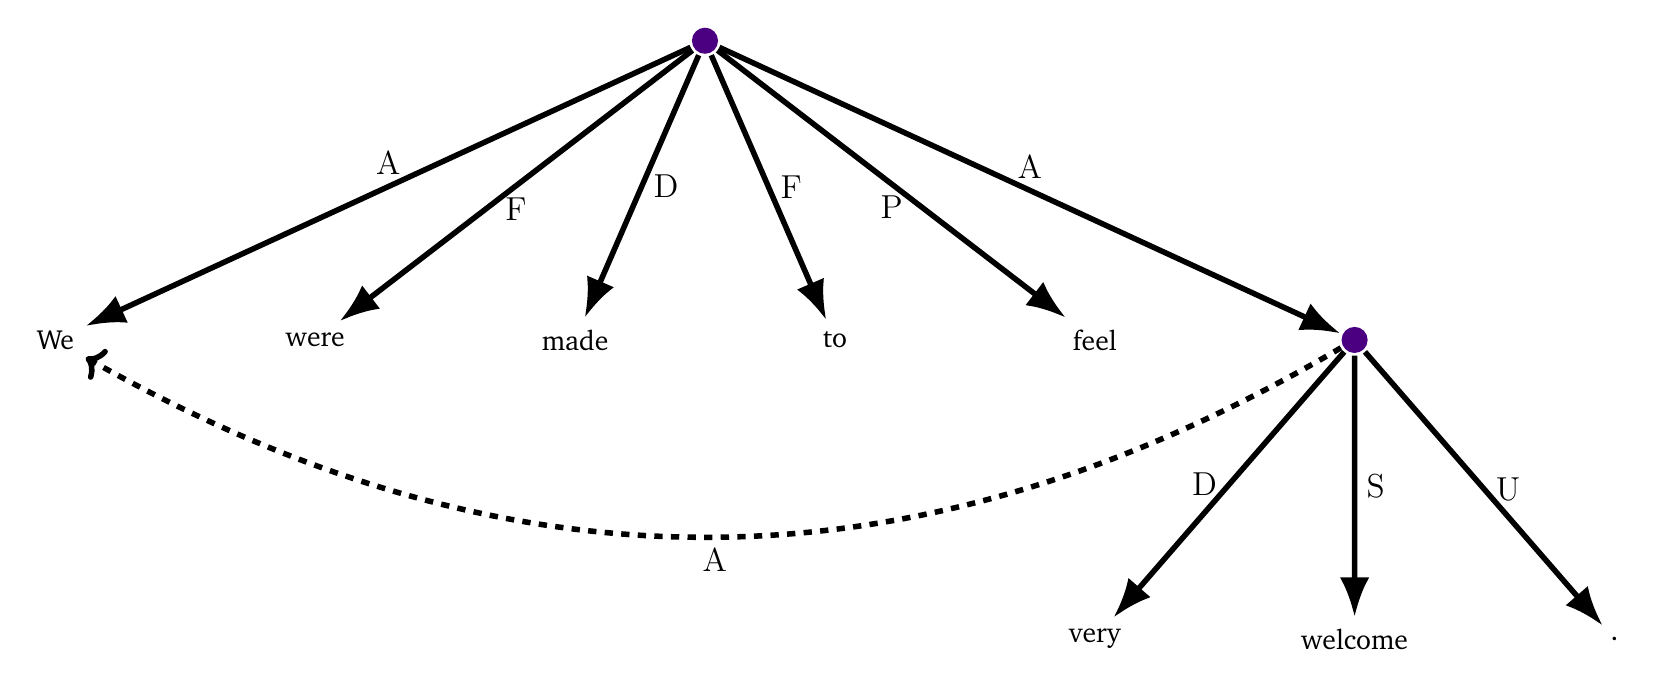
\begin{tikzpicture}[level distance=38mm,sibling distance=33mm, -{Latex[length=5mm]}, line width=2pt,
        every node/.append style={font=\large\bf\ttfamily},
        every circle node/.append style={fill=Indigo}]
      \tikzstyle{word} = [font=\rmfamily,color=black]
      \node (ROOT) [circle] {}
        child {node (We) [word] {We} edge from parent node[above] {A}}
        child {node [word] {were} edge from parent node[below] {F}}
        child {node [word] {made} edge from parent node[right] {D}}
        child {node [word] {to} edge from parent node[right] {F}}
        child {node [word] {feel} edge from parent node[below] {P}}
        child {node (verywelcome) [circle] {}
        {
          child {node [word] {very} edge from parent node[left] {D}}
          child {node [word] {welcome} edge from parent node[right] {S}}
          child {node [word] {.} edge from parent node[right] {U}}
        } edge from parent node[above] {A} }
      ;
      \draw[dashed,->,bend left] (verywelcome) to node [below] {A} (We);
    \end{tikzpicture}
  }
	\begin{adjustbox}{margin=3mm,frame,width=\textwidth}  \color{Indigo}
	\texttt{A}: participant \hspace{1cm} \texttt{F}: function \hspace{1cm} \texttt{D}: adverbial
	\hspace{1cm} \texttt{P}: process \hspace{1cm} \texttt{S}: state \hspace{1cm} \texttt{U}: punctuation
	\end{adjustbox}
  \captionof{figure}{\color{Indigo} Universal Conceptual Cognitive Annotation (UCCA).}
  \end{center}
\end{minipage}
\begin{minipage}{.45\columnwidth}
    \begin{center}
    \begin{dependency}[edge style={-{Latex[length=4mm]}, color=DarkBlue, line width=2pt},
        text only label, label style={above, color=DarkBlue, font=\bf\ttfamily}, font=\small]
   \begin{deptext}[column sep=.2em,ampersand replacement=\^]
    We \^ were \^ made \^ to \^ feel \^ very \^ welcome \^ . \\
    \end{deptext}
        \depedge[edge start x offset=1pt]{3}{1}{nsubj:pass}
        \depedge[edge below,dashed,edge unit distance=.65ex,edge end x offset=4pt]{5}{1}{nsubj:xsubj}
        \depedge[edge below,dashed,edge unit distance=.9ex,edge end x offset=-3pt]{7}{1}{nsubj:xsubj}
        \depedge[edge start x offset=-3pt]{3}{2}{aux:pass}
        \deproot[edge unit distance=3.4ex]{3}{root}
        \depedge{5}{4}{mark}
        \depedge[edge start x offset=3pt]{3}{5}{xcomp}
        \depedge{7}{6}{advmod}
        \depedge{5}{7}{xcomp}
        \depedge[edge unit distance=2ex,edge start x offset=-1pt]{3}{8}{punct}
    \end{dependency}
  \captionof{figure}{\color{DarkBlue} Universal Dependencies (UD).}
  \end{center}
\end{minipage}

\vfill
\hrule


\section*{Unified DAG Format}

We convert UD into a UCCA-like format supported by TUPA, by inserting non-terminal nodes.

\begin{minipage}{.4\columnwidth}
  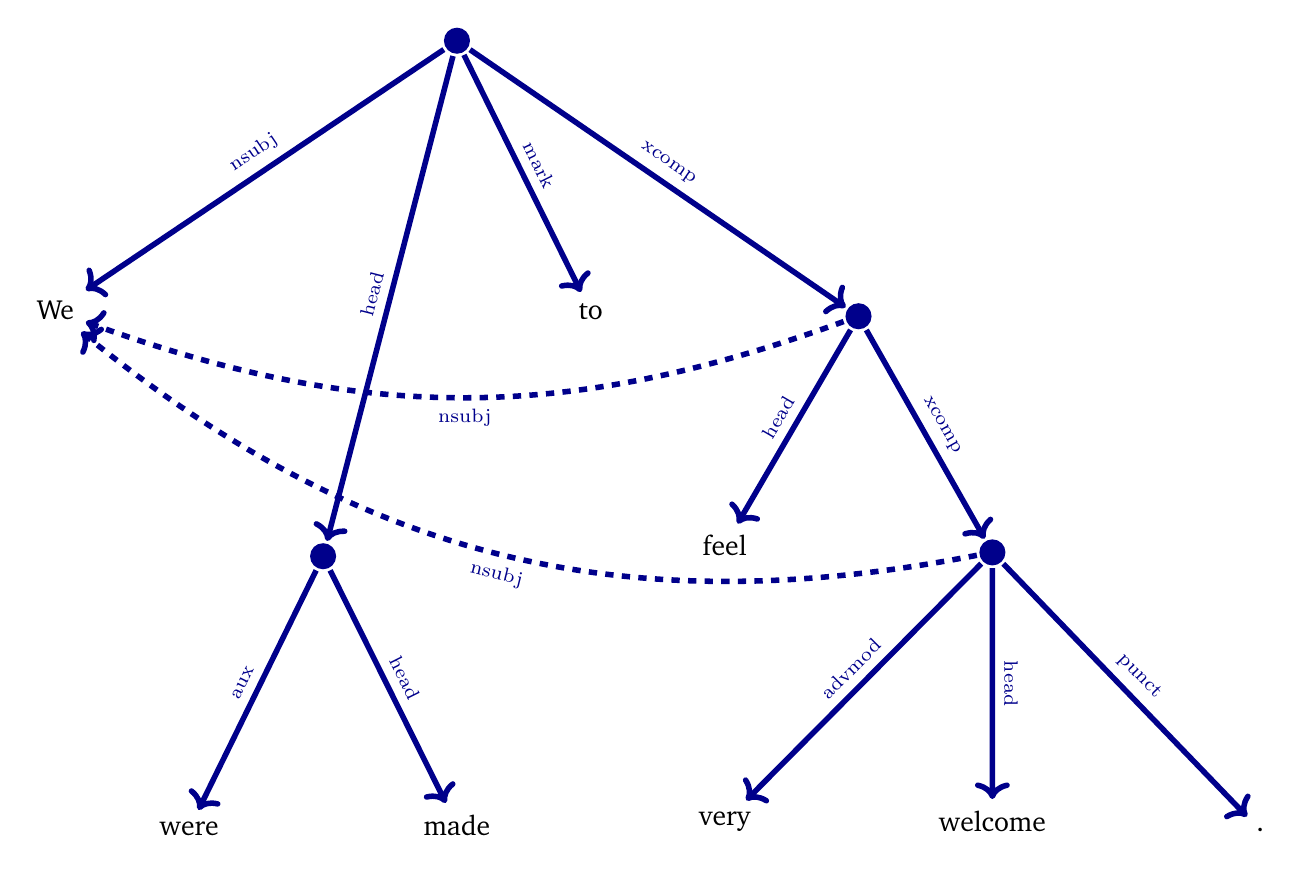
\begin{tikzpicture}[-{Latex[length=5mm]}, color=DarkBlue, line width=2pt,
      every node/.append style={sloped,anchor=south,auto=false,font=\scriptsize\bf\ttfamily},
      sibling distance=34mm, ->,
        every circle node/.append style={fill=DarkBlue},
        level 1/.style={level distance=37mm},
        level 2/.style={level distance=32mm},
        level 3/.style={level distance=37mm}]
      \tikzstyle{word} = [font=\rmfamily,color=black]
      \node (ROOT) [circle] {}
        child {node (We) [word] {We} edge from parent node[midway,above,sloped] {\scriptsize nsubj}}
        child {node {}
        {
	        child {node (weremade) [circle] {}
	        {
	          child {node [word] {were} edge from parent node[midway,above,sloped] {\scriptsize aux}}
	          child {node [word] {made} edge from parent node[midway,above,sloped] {\scriptsize head}}
	        } edge from parent [draw=none]}
        } edge from parent [draw=none]}
        child {node [word] {to} edge from parent node[midway,above,sloped] {\scriptsize mark}}
        child {node (feelverywelcome) [circle] {}
        {
          child {node [word] {feel} edge from parent node[midway,above,sloped] {\scriptsize head}}
          child {node (verywelcome) [circle] {}
          {
            child {node [word] {very} edge from parent node[midway,above,sloped] {\scriptsize advmod}}
            child {node [word] {welcome} edge from parent node[midway,above,sloped] {\scriptsize head}}
            child {node [word] {.} edge from parent node[midway,above,sloped] {\scriptsize punct}}
          } edge from parent node[midway,above,sloped] {\scriptsize xcomp} }
        } edge from parent node[midway,above,sloped] {\scriptsize xcomp} }
      ;
      \draw[->] (ROOT) to node [midway,above,sloped] {\scriptsize head} (weremade);
      \draw[dashed,->,bend left=25] (verywelcome) to node [midway,below,sloped] {\scriptsize nsubj} (We);
      \draw[dashed,->,bend left=20] (feelverywelcome) to node [midway,below,sloped] {\scriptsize nsubj} (We);
  \end{tikzpicture}
\end{minipage}
\hfill
\begin{minipage}{.5\columnwidth}
    \scalebox{.8}{
	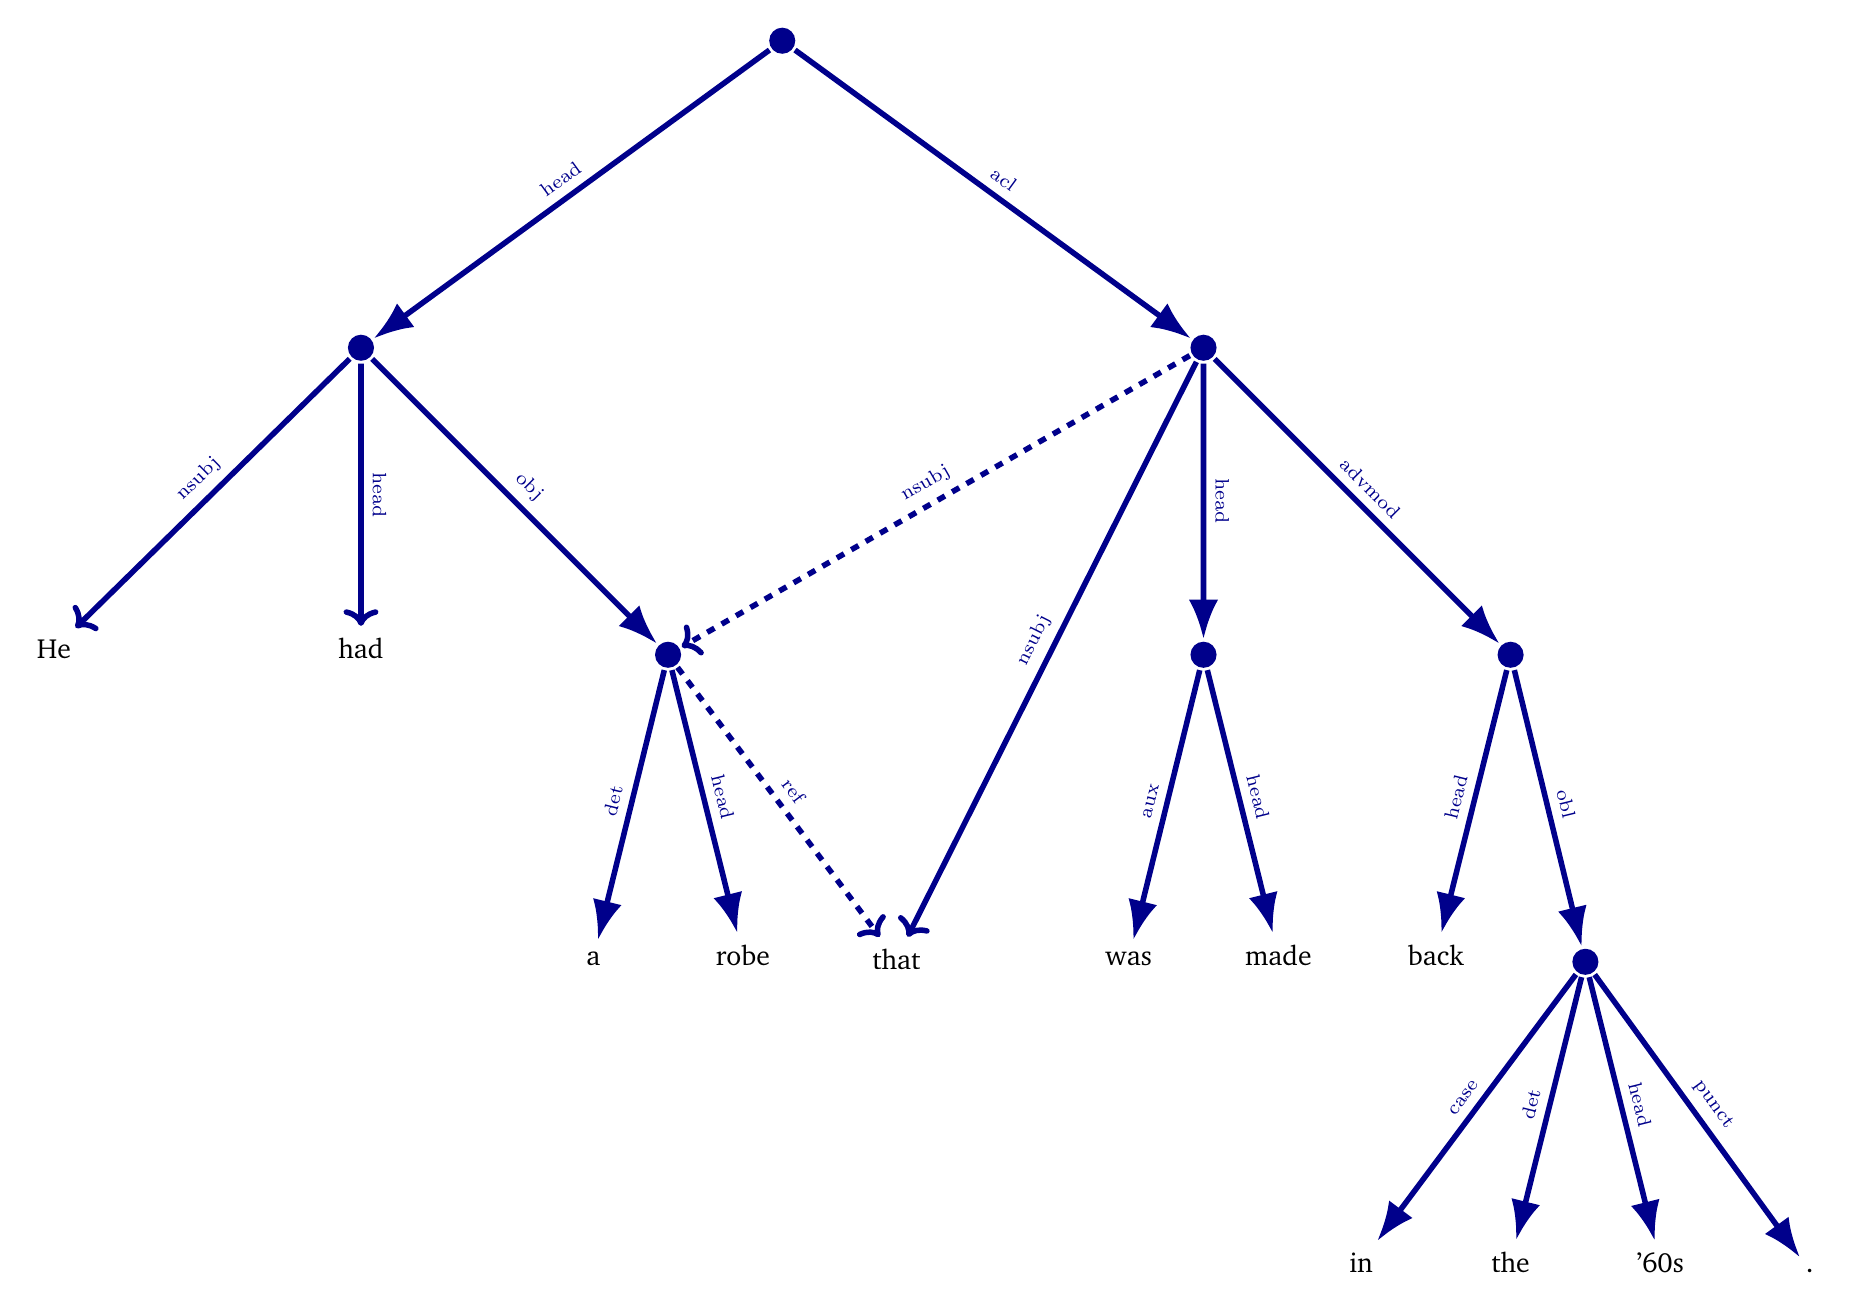
\begin{tikzpicture}[-{Latex[length=5mm]}, color=DarkBlue, line width=2pt,
      every node/.append style={sloped,anchor=south,auto=false,font=\scriptsize\bf\ttfamily},
      level distance=41mm,
	  level 1/.style={sibling distance=107mm},
	  level 2/.style={sibling distance=39mm},
	  level 3/.style={sibling distance=19mm},
	  level 4/.style={sibling distance=19mm},
	  every circle node/.append style={fill=DarkBlue}]
	  \tikzstyle{word} = [font=\rmfamily,color=black]
	  \node (1_1) [circle] {}
	  {
	  child {node (1_2) [circle] {}
	    {
	    child {node (1_6) [word] {He}  edge from parent [draw=none]}
	    child {node (1_3) [word] {had}  edge from parent [draw=none]}
	    child {node (1_7) [circle] {}
	      {
	      child {node (1_14) [word] {a}  edge from parent node[midway,above,sloped]  {\scriptsize det}}
	      child {node (1_8) [word] {robe}  edge from parent node[midway,above,sloped]  {\scriptsize head}}
	      } edge from parent node[midway,above,sloped]  {\scriptsize obj}}
	    } edge from parent node[midway,above,sloped]  {\scriptsize head}}
	  child {node (1_4) [circle] {}
	    {
	    child {node {}
	    {
    	    child {node (1_15) [word] {that}  edge from parent [draw=none]}
    	} edge from parent [draw=none]}
	    child {node (1_5) [circle] {}
	      {
	      child {node (1_9) [word] {was}  edge from parent node[midway,above,sloped]  {\scriptsize aux}}
	      child {node (1_10) [word] {made}  edge from parent node[midway,above,sloped]  {\scriptsize head}}
	      } edge from parent node[midway,above,sloped]  {\scriptsize head}}
	    child {node (1_11) [circle] {}
	      {
	      child {node (1_12) [word] {back}  edge from parent node[midway,above,sloped]  {\scriptsize head}}
	      child {node (1_16) [circle] {}
	        {
	        child {node (1_18) [word] {in}  edge from parent node[midway,above,sloped]  {\scriptsize case}}
	        child {node (1_19) [word] {the}  edge from parent node[midway,above,sloped]  {\scriptsize det}}
	        child {node (1_17) [word] {'60s}  edge from parent node[midway,above,sloped]  {\scriptsize head}}
	        child {node (1_20) [word] {.}  edge from parent node[midway,above,sloped]  {\scriptsize punct}}
	        } edge from parent node[midway,above,sloped]  {\scriptsize obl}}
	      } edge from parent node[midway,above,sloped]  {\scriptsize advmod}}
	    } edge from parent node[midway,above,sloped]  {\scriptsize acl}}
	  };
	  \draw[->] (1_2) to node [midway,above,sloped] {\scriptsize nsubj} (1_6);
	  \draw[->] (1_2) to node [midway,above,sloped] {\scriptsize head} (1_3);
	  \draw[->] (1_4) to node [midway,above,sloped] {\scriptsize nsubj} (1_15);
	  \draw[dashed,->] (1_4) to node [midway,above,sloped] {\scriptsize nsubj} (1_7);
	  \draw[dashed,->] (1_7) to node [midway,above,sloped] {\scriptsize ref} (1_15);
	\end{tikzpicture}}
\end{minipage}


\columnbreak



\section*{Enhanced Dependencies}

\begin{adjustbox}{width=\columnwidth,margin=3pt,frame}
\texttt{1 We we PRON PRP Case=Nom|Number=Plur|Person=1|PronType=Prs 3 nsubj:pass 3:nsubj:pass|5:nsubj:xsubj|7:nsubj:xsubj \textunderscore}
\end{adjustbox}


UD graph from \verb|reviews-341397-0003| (\verb|UD_English-EWT|),
containing conjoined predicates and arguments:

    \begin{dependency}[text only label, label style={above}, font=\small]
    \begin{deptext}[column sep=1em,ampersand replacement=\^]
    he \^ went \^ straight \^ to \^ work \^ and \^ finished \^ the \^ job \^ efficiently \^ and \^ promptly \^ ! \\
    \end{deptext}
        \depedge[edge start x offset=1pt]{2}{1}{nsubj}
        \depedge[edge below,dashed,edge unit distance=.5ex,edge end x offset=2pt]{7}{1}{nsubj}
        \deproot[edge unit distance=3ex]{2}{root}
        \depedge[edge start x offset=3pt]{2}{3}{advmod}
        \depedge{5}{4}{mark}
        \depedge[edge unit distance=1.75ex,edge start x offset=2pt]{2}{5}{advcl}
        \depedge{7}{6}{cc}
        \depedge[edge unit distance=1.5ex,edge start x offset=1pt]{2}{7}{conj}
        \depedge{9}{8}{det}
        \depedge[edge unit distance=2.5ex,edge start x offset=1pt]{7}{9}{obj}
        \depedge[edge unit distance=2.5ex,edge start x offset=-1pt]{7}{10}{advmod}
        \depedge{12}{11}{cc}
        \depedge{10}{12}{conj}
        \depedge[edge below,dashed,edge unit distance=.65ex,edge end x offset=2pt]{7}{12}{advmod}
        \depedge[edge unit distance=1ex,edge start x offset=-1pt]{2}{13}{punct}
    \end{dependency}
    
{\small\verb|newsgroup-groups.google.com_GuildWars_086f0f64ab633ab3_ENG_20041111_173500-0051|} (\verb|UD_English-EWT|), containing a null node (\textbf{E9.1}) and
case information (nmod:on):

    \begin{dependency}[text only label, label style={above}, font=\small]
    \begin{deptext}[column sep=1.2em,ampersand replacement=\^]
    I \^ wish \^ all \^ happy \^ holidays \^ , \^ and \^ moreso \^ , \^ \textbf{E9.1} \^ peace \^ on \^ earth \^ . \\
    \end{deptext}
        \depedge[edge start x offset=1pt]{2}{1}{nsubj}
        \deproot[edge start x offset=-1pt,edge unit distance=3ex]{2}{root}
        \depedge[edge start x offset=3pt]{2}{3}{iobj}
        \depedge{5}{4}{amod}
        \depedge[edge start x offset=2pt]{2}{5}{obj}
        \depedge[edge unit distance=2ex]{11}{6}{punct}
        \depedge[edge start x offset=4pt,edge below,dashed]{10}{6}{punct}
        \depedge[edge start x offset=-1pt,edge unit distance=1.85ex]{11}{7}{cc}
        \depedge[edge start x offset=1pt,edge below,dashed]{10}{7}{cc}
        \depedge[edge start x offset=-3pt,edge unit distance=1.5ex]{11}{8}{orphan}
        \depedge[edge start x offset=-1pt,edge below,dashed]{10}{8}{advmod}
        \depedge[edge start x offset=-5pt,edge unit distance=.8ex]{11}{9}{punct}
        \depedge[edge start x offset=-3pt,edge below,dashed]{10}{9}{punct}
        \depedge[edge unit distance=1.45ex]{2}{11}{conj}
        \depedge[edge below,dashed]{10}{11}{obj}
        \depedge{13}{12}{case}
        \depedge[edge start x offset=1pt]{11}{13}{nmod}
        \depedge[edge start x offset=-1pt,edge unit distance=1.35ex]{2}{14}{punct}
    \end{dependency}
    
\verb|reviews-255261-0007| (\verb|UD_English-EWT|), containing a relative clause:

    \begin{dependency}[text only label, label style={above}, font=\small]
    \begin{deptext}[column sep=.1em,ampersand replacement=\^]
    He \^ had \^ a \^ robe \^ that \^ was \^ made \^ back \^ in \^ the \^ '60s \^ . \\
    \end{deptext}
        \depedge[edge start x offset=1pt]{2}{1}{nsubj}
        \deproot[edge start x offset=-1pt,edge unit distance=3.355ex]{2}{root}
        \depedge{4}{3}{det}
        \depedge{2}{4}{obj}
        \depedge[edge unit distance=1.5ex,edge below,dashed]{7}{4}{nsubj:pass}
        \depedge[edge start x offset=2pt]{7}{5}{nsubj:pass}
        \depedge[edge start x offset=4pt,edge below,dashed]{4}{5}{ref}
        \depedge[edge unit distance=2ex]{7}{6}{aux:pass}
        \depedge[edge start x offset=-1pt,edge unit distance=2.75ex]{4}{7}{acl:relcl}
        \depedge[edge start x offset=-3pt]{7}{8}{advmod}
        \depedge{11}{9}{case}
        \depedge{11}{10}{det}
        \depedge[edge unit distance=1ex,edge below,dashed]{8}{11}{obl}
        \depedge[edge start x offset=-1pt,edge unit distance=1.2ex]{2}{12}{punct}
    \end{dependency}

    
    
The same graph after conversion to the unified DAG format.
The cycle is removed due to the non-terminal nodes introduced in the conversion.


\hrule


\section*{Results}

Aggregated test LAS-F1 scores
for our system (TUPA) and the baseline system (UDPipe 1.2):
\begin{tabular}{lccc}
& \multirow{2}{32mm}{\bf TUPA {\small(official)}} & \multirow{2}{35mm}{\bf TUPA {\small(unofficial)}}
& \multirow{2}{34mm}{\bf UDPipe {\small(baseline)}} \\\\
All treebanks & 53.69 & 58.48 & 65.80 \\
Big treebanks & 62.07 & 67.36 & 74.14 \\
PUD treebanks & 56.35 & 56.82 & 66.63 \\
Small treebanks & 36.74 & 41.19 & 55.01 \\
Low-resource & 8.53 & 12.68 & 17.17
\end{tabular}


{
\setlength{\columnsep}{5mm}
\setlength{\columnseprule}{0pt}
\begin{multicols}{2}
\color{DarkSlateGray}
\tiny\titleformat*{\section}{\small}
\bibliographystyle{plain}
\bibliography{references}

\color{Black}
\begin{adjustbox}{margin=3mm,frame,minipage=1.1\columnwidth}
\centering\large
Please join SemEval 2019 Task 1: \\
Cross-lingual Semantic Parsing with UCCA

\begin{minipage}{.3\textwidth}
\includegraphics[width=\textwidth]{qr}\end{minipage}
\hfill
\begin{minipage}{.6\textwidth}\Large\url{tinyurl.com/semeval-ucca}\end{minipage}
\end{adjustbox}
\end{multicols}
}

\end{multicols}

\catcode`\_=12
\pgfplotstableread{
corpus
af_afribooms
grc_perseus
grc_proiel
ar_padt
hy_armtdp
eu_bdt
br_keb
bg_btb
bxr_bdt
ca_ancora
hr_set
cs_cac
cs_fictree
cs_pdt
cs_pud
da_ddt
nl_alpino
nl_lassysmall
en_ewt
en_gum
en_lines
en_pud
et_edt
fo_oft
fi_ftb
fi_pud
fi_tdt
fr_gsd
fr_sequoia
fr_spoken
gl_ctg
gl_treegal
de_gsd
got_proiel
el_gdt
he_htb
hi_hdtb
hu_szeged
zh_gsd
id_gsd
ga_idt
it_isdt
it_postwita
ja_gsd
ja_modern
kk_ktb
ko_gsd
ko_kaist
kmr_mg
la_ittb
la_perseus
la_proiel
lv_lvtb
pcm_nsc
sme_giella
no_bokmaal
no_nynorsk
no_nynorsklia
fro_srcmf
cu_proiel
fa_seraji
pl_lfg
pl_sz
pt_bosque
ro_rrt
ru_syntagrus
ru_taiga
sr_set
sk_snk
sl_ssj
sl_sst
es_ancora
sv_lines
sv_pud
sv_talbanken
th_pud
tr_imst
uk_iu
hsb_ufal
ur_udtb
ug_udt
vi_vtb
}\corpus
    \begin{tikzpicture}
    \begin{axis}[
    ybar=0pt,  
    enlarge x limits={0.01},
    enlarge y limits={value=0.1,upper},
    ymin=0,
    width=1.04\textwidth,
    height=18cm,
    bar width=10pt,
    xtick=data,
    xticklabels from table={\corpus}{corpus},
    xticklabel style={font=\tiny,rotate=75,anchor=east},
    xtick align=inside,
    xticklabel pos=left,
    yticklabels=none,
    tickwidth=0pt,
    legend style={at={(axis cs:0.5,90)},anchor=north west},
    legend cell align={left},
    nodes near coords={
     \scalebox{.6}{\pgfmathprintnumber[precision=2]{\pgfplotspointmeta}}
    },
    every node near coord/.append style={rotate=90,anchor=west},
    axis background/.style={fill=lightgray!50}
    ]
    \addplot[fill=red]table[x expr=\coordindex,meta=corpus,y=test]{udst2018scores.txt};
    \addplot[fill=blue]table[x expr=\coordindex,meta=corpus,y=enhanced]{udst2018scores.txt};
    \legend{Basic,Enhanced}
    \end{axis}
    \end{tikzpicture}
\catcode`\_=8

\end{document}
